\begin{definition}[Local Maximum, Local Minimum] \leavevmode\\
    Let $\emptyset \not = A \subseteq (X, d),$ and let $f:A \to \R.$
    \begin{enumerate}[$(i)$]
        \item We say that $f$ has a local maximum at $c \in A$ if
        $$
        \exists \delta > 0 \st \forall x \in \nbhd{\delta}{c}\cap A ~~f(x)\leq f(c)
        $$
        \item We say that $f$ has a local minimum at $c \in A$ if 
        $$
        \exists \delta > 0 \st \forall x \in \nbhd{\delta}{c}\cap A ~~f(x) \geq f(c)
        $$
    \end{enumerate}
\end{definition}

\begin{lemma}[Order Limit Theorem for Functions] \leavevmode\\
    Suppose $\lims{x}{c}g(x)$ and $\lims{x}{c}h(x)$ both exist.
    \begin{enumerate}[$(i)$]
    \item If $\exists \delta > 0 \st \forall x \in (c-\delta, c) ~~h(x) \leq g(x),$ then $\lims{x}{c}h(x) \leq \lims{x}{c}g(x)$
    \item If $\exists \delta > 0 \st \forall x \in (c, c + \delta) ~~h(x) \leq g(x),$ then $\lims{x}{c}h(x) \leq \lims{x}{c}g(x)$
    \end{enumerate}
\end{lemma}

\begin{proof}
    Here we will prove $(i)$. The proof of $(ii)$ is analogous. Let $(a_n)$ be a sequence in $(c-\delta, c)$ such that $a_n \to c.$ By the sequential criterion for limits of functions we have
    \begin{equation}
        a_n \to c \implies \begin{cases*}
            \lims{n}{\infty}g(a_n) = \lims{x}{c}g(x) \\
            \lims{n}{\infty}h(a_n) = \lims{x}{c}h(x)
        \end{cases*}
        \tag{$I$}
    \end{equation}
    Also note that
    \begin{align*}
        \forall n ~~a_n\in (c-\delta, c) &\implies \forall n ~~h(a_n) \leq g(a_n) \\
        &\overset{\text{OLTS}}{\implies} \lims{n}{\infty}h(a_n) \leq \lims{n}{\infty}g(a_n) \tag{$II$}
    \end{align*}
    It follows from $(I),(II)$ that $\lims{x}{c}h(x) \leq \lims{x}{c}g(x).$ \qed
\end{proof}

\begin{theorem}[Interior Extremum Theorem] \leavevmode\\
    \label{Thm5.8}
    Let $I\subseteq \R$ be an interval, $f:I \to \R$ be a function and $c \in \closure{I}.$ Suppose $f$ is differentiable at $c$. Then
    \begin{enumerate}[$(i)$]
        \item If $f$ has a local maximum at $c$, then $f'(c) = 0$
        \item If $f$ has a local minimum at $c$, then $f'(c) = 0$
    \end{enumerate}
\end{theorem}

\begin{proof}
    Here, we will prove $(i)$. The proof for $(ii)$ is analogous. Suppose $f$ has a local maximum at $c$.
    \begin{enumerate}
        \item $f$ has a local maximum at $c \implies \exists \delta_1 \st \forall x \in (c - \delta_1, c+ \delta_1) \cap I ~~f(x) \leq f(c)$
        \item $c$ is an interior point of $I\implies \exists \delta_2 \st (c-\delta_2, c+\delta_2) \subseteq I$
    \end{enumerate}
    So, if we let $\delta = \min \{\delta_1, \delta_2\}$, then
    $$
    \forall x \in (c-\delta, c+\delta) ~~f(x) \leq f(c)
    $$
    We have
    \begin{enumerate}[$(I)$]
        \item For all $x\in (c-\delta, c)$
        \begin{align*}
            \begin{rcases*}
                x -c < 0 \\
                f(x) \leq f(c)
            \end{rcases*} &\implies \slope{f(x)}{f(c)}{x}{c} \geq 0 \\
            &\overset{OLTF}{\implies} \deriv{f}{c} \geq \lims{x}{c} 0 \\
            &\implies f'(c) \geq 0.
        \end{align*}

        \item For all $x\in (c, c+\delta)$
        \begin{align*}
            \begin{rcases*}
                x -c > 0 \\
                f(x) \leq f(c)
            \end{rcases*} &\implies \slope{f(x)}{f(c)}{x}{c} \leq 0 \\
            &\overset{OLTF}{\implies} \deriv{f}{c} \leq \lims{x}{c} 0 \\
            &\implies f'(c) \leq 0.
        \end{align*}
    \end{enumerate}
    It follows from $(I),(II)$ that $f'(c) = 0$. \qed
\end{proof}

\begin{remark}
    The following are three techniques that can be used in proving the existence of a solution:
    \begin{enumerate}
        \item Suppose $h:[a,b] \to \R$ is continuous. Let $\alpha$ be a given real number. One way to show there exists a number $c$ such that $h(c) = \alpha$ is as follows:
        $$
        \text{Prove that $m \leq \alpha \leq M$ where }
        \begin{cases*}
            m = \min \{h(x) : x \in [a,b]\} \\
            M = \max \{h(x) : x \in [a,b]\}
        \end{cases*}
        $$

        \item Suppose $g:[a,b] \to \R$ is differentiable. One way to prove that there exists a number $c$ such that $g'(c) = 0$ is as follows:
        $$
        \text{Prove there is a point in $(a,b)$ at which $g$ has a local maximum or a local minimum}
        $$

        \item Suppose $h:[a,b] \to \R$ is differentiable. Let $\alpha$ be a given real number. One way to prove that there exists a number $c$ such that $h'(c) = \alpha$ is as follows:
        $$
        \text{Define $g(x)=h(x) - \alpha x$ and prove that there is a point $c$ at which $g'(c) = 0$}
        $$
    \end{enumerate}
\end{remark}

\begin{theorem}[Darboux's Theorem] \leavevmode\\
    \label{Thm5.12}
    Suppose $f:[a,b] \to \R$ is differentiable such that $f'(a) < f'(b)$ (or $f'(b) < f'(a)$), and let $\alpha \in \R$ be such that $f'(a) < \alpha < f'(b)$ (or $f'(b) < \alpha < f'(a)$). Then
    $$
    \exists c \in (a,b) \st f'(c) = \alpha
    $$
\end{theorem}

\begin{proof}
    Let $g:[a,b] \to \R$ be defined by $g(x) = f(x) - \alpha x.$ It follows from the algebraic differentiability theorem that $g$ is differentiable on $[a,b]$, and so it is continuous on $[a,b]$. It is enough to show that
    $$
    \exists c \in (a,b) \st g'(c) = 0
    $$
    To this end, it is enough to show that $\exists c \in (a,b)$ at which $g$ has a local minimum. We have
    $$
    \begin{rcases*}
        \text{$g$ is continuous on [a,b]} \\
        \text{$[a,b]$ is compact}
    \end{rcases*} \implies
    \text{$g$ attains its minimum on $[a,b]$}
    $$
    Let $\hat{c}$ be a point at which $g$ attains a minimum. In what follows we will show that $\hat{c}\in (a,b)$ and so it can be used as the $c$ that we were looking for. Note that (since $g'(x) = f'(x) - \alpha$)
    \begin{align*}
        g'(a) = f'(a) - \alpha < 0 \\
        g'(b) = f'(b) - \alpha > 0
    \end{align*}

    \begin{description}
        \item[Claim 1: $\hat{c} \not = a$ ]\leavevmode \\
        Assume for contradiction that $\hat{c} = a$. Then
        $$
        \forall x \in [a, b] ~~g(x) \geq g(a)
        $$
        so,
        $$
        \forall x \in [a,b] ~~\begin{cases*}
            g(x) - g(a) \geq 0 \\
            x-a > 0
        \end{cases*}
        $$
        Thus
        $$
        \forall x \in (a, b) ~~\slope{g(x)}{g(a)}{x}{a} \geq 0
        $$
        Thus
        $$
        \deriv{g}{a} \geq \lims{x}{a}0
        $$
        That is, $g'(a) \geq 0.$ This contradicts the fact that $g'(a) < 0$.
        \item[Claim 2: $\hat{c} \not = b$] \leavevmode\\
        Assume for contradiction that $\hat{c} = b$.
        In a similar manner to claim 1:
        \begin{align*}
            \forall x \in [a,b] ~~g(x) \geq g(b) 
            &\implies \forall x \in [a,b] ~~\begin{cases*}
                g(x) - g(b) \geq 0 \\
                x - b < 0
            \end{cases*} \\
            &\implies \forall x \in [a,b] ~~\slope{g(x)}{g(b)}{x}{b} \leq 0
        \end{align*}
        Thus,
        $$
        \deriv{g}{b} \leq \lims{x}{b}0
        $$
        That is,
        $$
        g'(b) \leq 0.
        $$
        This contradicts the fact that $g'(b) > 0.$
    \end{description}
\end{proof}

\begin{example}
    Does there exist a differentiable function $f:[-1,1] \to \R$ whose derivative is $H: [-1,1] \to \R$ defined by
    $$
    H(x) = \begin{cases*}
        1 &$0 \leq x \leq 1$ \\
        0 &$-1 \leq x \leq 0$
    \end{cases*}?
    $$
    No! $H$ does not have the intermediate value property. So, it cannot be the derivative of any differentiable function.
\end{example}

The following are some geometric conjectures involving the derivative of a function.

\begin{conjecture}\leavevmode\\
\label{Conj1}
Suppose $f:[a,b] \to \R$ is differentiable. Suppose $f(a) = f(b)$. Then there exists a point $c\in (a,b)$ at which the tangent line is horizontal. I.e., there exists $c\in(a,b) \st f'(c) = 0$.
\end{conjecture}

\begin{figure}[h]
    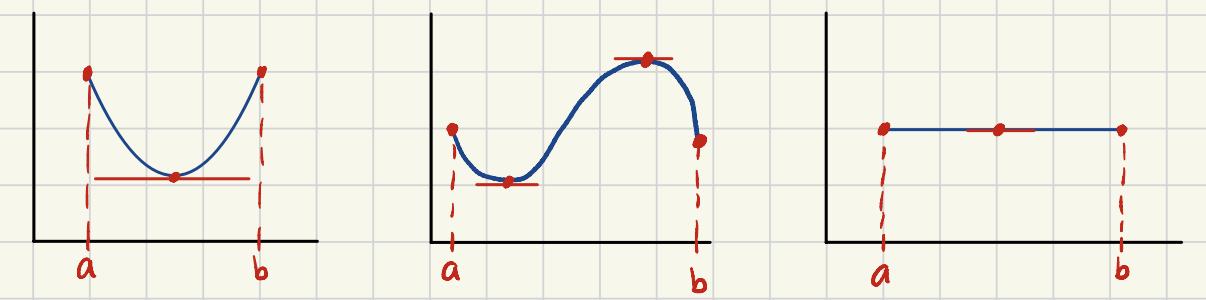
\includegraphics[width=.75\linewidth, center]{/Users/josiahvillarante/GradSchool/Grad-School-Notes/Math230B/Lecture/CH5/images/Conjecture1.png}
\end{figure}

\begin{conjecture}\leavevmode\\
\label{Conj2}
Suppose $f:[a,b] \to \R$ is differentiable. Then there exists a point $c \in (a,b)$ at which the tangent line is parallel to the line through the endpoints $(a, f(a))$ and $(b, f(b))$. I.e., there exists $c \in (a,b) \st f'(c) = \slope{f(b)}{f(a)}{b}{a}.$
\end{conjecture}

\begin{figure}[h!]
    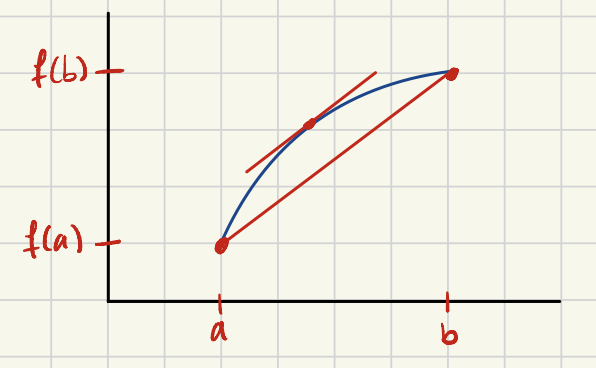
\includegraphics[width=.25\linewidth, center]{/Users/josiahvillarante/GradSchool/Grad-School-Notes/Math230B/Lecture/CH5/images/Conjecture2.png}
\end{figure}

\begin{conjecture}\leavevmode \\
\label{Conj3}
Suppose $\vec{r}: [a,b] \to \R^2, ~\vec{r}(t) = \left(f(t), g(t)\right)$ is a differentiable path in $\R^2$. Then there exists a point $\vec{r}(c)$ on the curve at which the tangent line is parallel to the line through the endpoints $\vec{r}(a)$ and $\vec{r}(b)$. Let's try to find a mathematical formula for this statement:
    \begin{enumerate}[$*)$]
        \item The direction vector for the tangent line at the point $\vec{r}(c): ~\vec{r}'(c) = \left(f'(c), g'(c)\right)$
        \item The direction vector for the line through the endpoints: $\left(f(b) - f(a), g(b) - g(a)\right)$
    \end{enumerate}
So, assuming these vectors are nonzero, the claim of the conjecture can be described mathematically as
$$
    \exists c \exists \lambda \in \R \backslash \{0\} \st \left(f'(c), g'(c)\right) = \lambda \left(f(b) - f(a), g(b) - g(a)\right)
$$
Note that
\begin{align*}
    (f'(c), g'(c)) &= \lambda \left(f(b) - f(a), g(b) - g(a)\right) \\ 
    &\implies \begin{cases*}
        f'(c) = \lambda \left(f(b) - f(a)\right) \\
        g'(c) = \lambda \left(g(b) - g(a)\right)
    \end{cases*} \\
    &\implies \lambda f'(c)\left[g(b) - g(a)\right] = \lambda g'(c) \left[f(b) - f(a)\right] \\
    &\implies f'(c) \left[f(b) - f(a) \right] = g'(c) \left[g(b) - g(a)\right]
\end{align*}
\end{conjecture}